\chapter{Approaches}\label{ch:approaches}

At this stage, we are going to propose a software development approach to tackle the problem. Running seL4 applications in Linux requires introducing an extra compatibility layer between the application and the Linux OS. Hence we are going to propose two approaches to achieve this: the API layer emulation approach and the ABI layer emulation approach.  

\section{API Layer Emulation Approach}

In the original seL4 system, a userland seL4 client application can request OS services from another seL4 server application which also runs in the userland through IPC mechanisms provided by the seL4 kernel. The seL4 system call library provides abstractions to those IPC interfaces.

% (Fixed: How does this related to the background?)

However, if those seL4 userland applications run on top of Linux OS, then directly using the original seL4 system call libraries will not work due to the different semantics between seL4 and Linux. To solve that problem, Cygwin gives a good idea. In Cygwin, it replaces the original system call libraries with a custom implementation to achieve compatibility between POSIX and Windows. Hence, we can provide a custom system call library that exports the same interfaces as the original seL4 system call libraries to seL4 userland applications, but we will use Linux IPC mechanisms as a replacement instead of invoking the seL4 IPC directly.

\subsection{ Design Model}

Figure \ref{fig:mapi} shows the model of the API layer emulation approach. 

\begin{figure}[h]
    \centering
    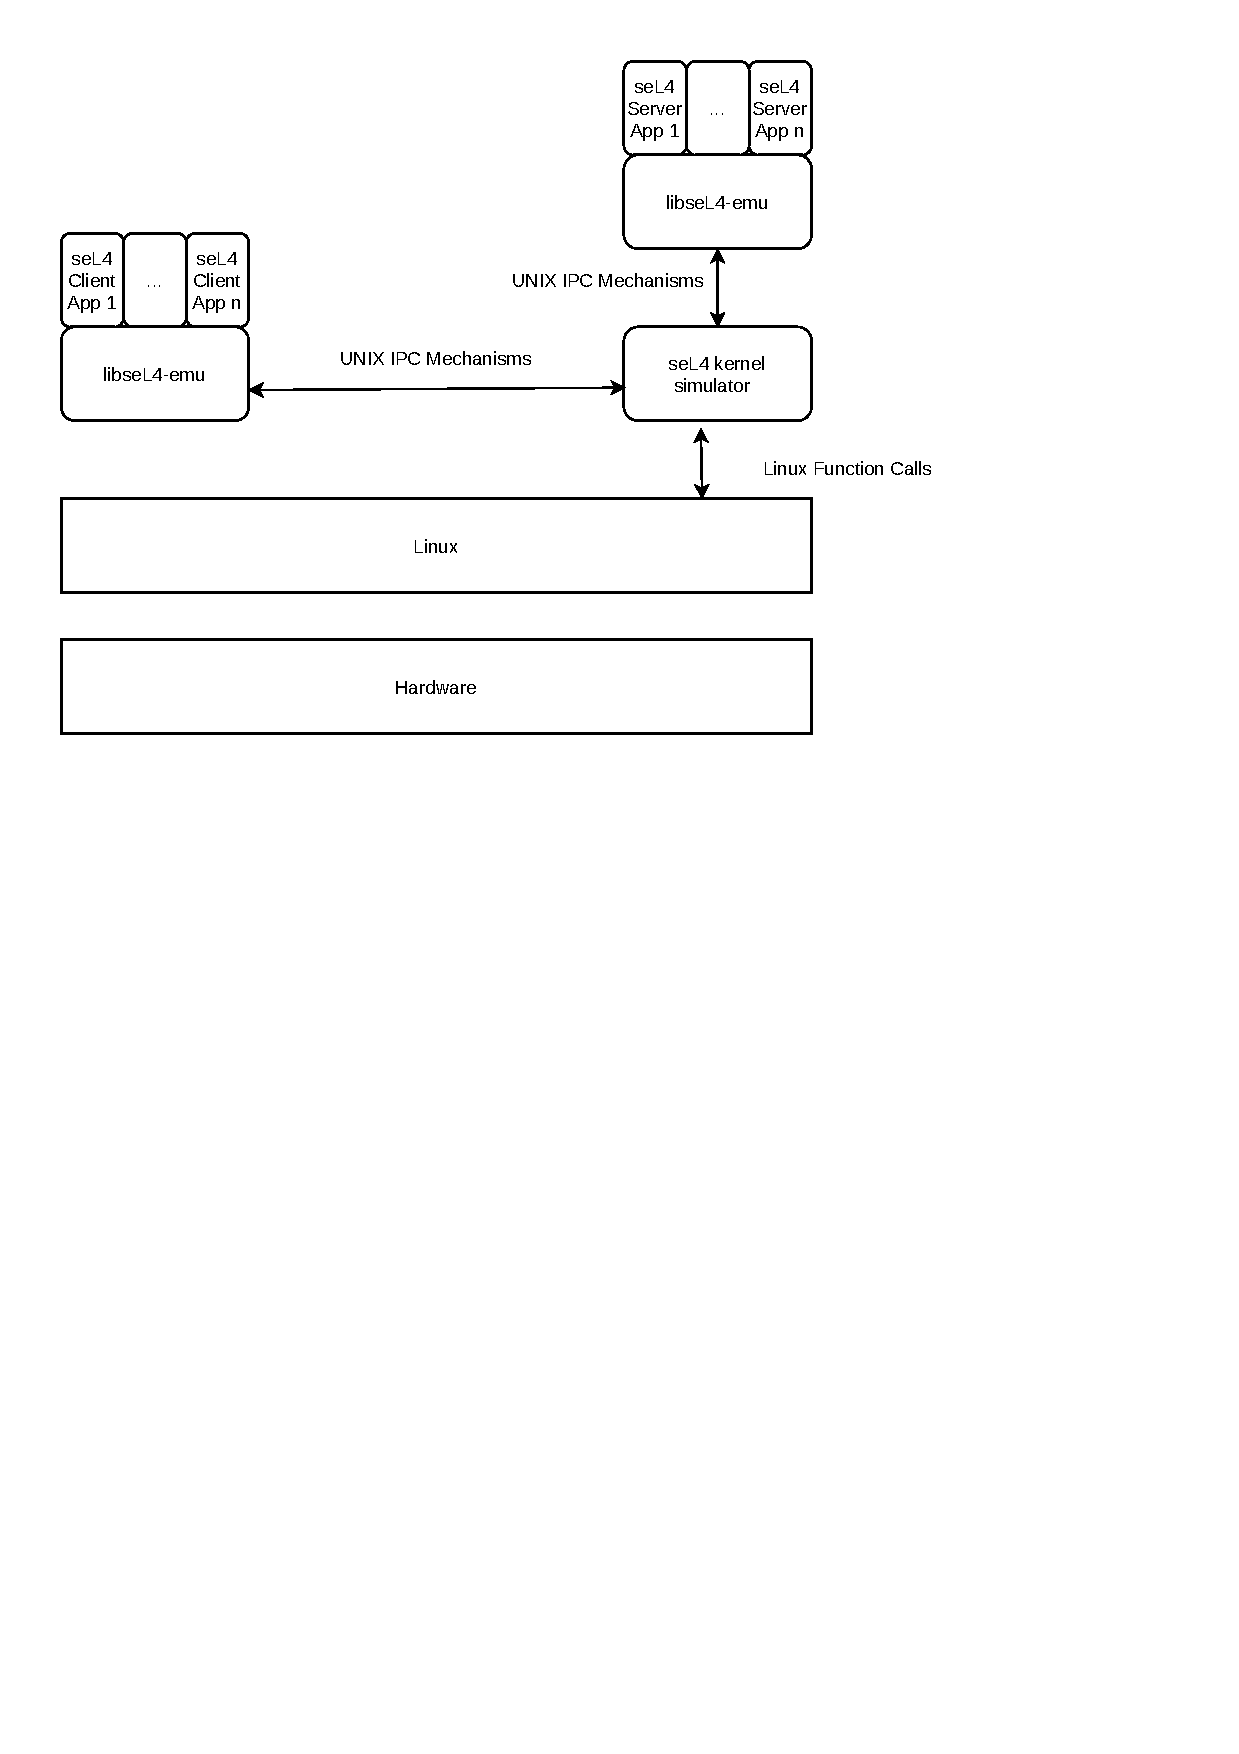
\includegraphics[clip, trim=0.5cm 16cm 3cm 0.5cm, width=0.9\textwidth, height=0.8\textwidth]{ch3/model1-v3.pdf}
    \caption{The model of API layer emulation approach}
    \label{fig:mapi}
\end{figure}

In general we need to develop two components in this model. 

\begin{enumerate}
\item An seL4 emulation library
\item An seL4 kernel simulator
\end{enumerate}

The seL4 emulation library is a compatibility layer named libseL4-emu in the figure which can be linked to other seL4 applications. Therefore, the seL4 applications will invoke the emulated seL4 system calls instead of the real original seL4 system calls. And the libseL4-emu library will dispatch those system call requests to the seL4 kernel simulator. 

The seL4 kernel simulator is a regular user-level Linux application. Hence the emulated seL4 applications can communicate with the seL4 kernel simulator using Linux IPC, such as UDS or shared memory. The seL4 kernel simulator mainly provides the seL4 semantics and management of capability space, IPC mechanisms, scheduling context management, etc. 

In this model, all the seL4 applications and the seL4 kernel simulator are just regular Linux processes running at the user level. The seL4 applications act as clients, communicating with the server which is our seL4 kernel simulator. 

\subsection{Advantages and Disadvantages}

The API layer emulation approach has several advantages. First of all, it is relatively easy to implement regarding the complexity of implementation.

% (Fixed: explain why the performance should be good? Comparing to Virtualization/ Emulation? VM exit/ VM_enter, IPC heavy/light? Context Switches in this approached requires 4 traps, native seL4 requires 2 traps) 

Secondly, since simulating the seL4 IPC mechanisms uses Linux IPC mechanisms won't introduce too much overhead, the performance should be relatively good compared to fully emulating a machine using QEMU. But it's hard to give an intuitive result of comparing this approach with the hardware virtualization approach using QEMU without further detailed measurement. Although the hardware virtualization will introduce the overhead due to the word switching, the API layer emulation approach will require at least four context switches between the seL4 client application, the seL4 kernel simulator, and the seL4 server application.

Whatsmore, this approach is ISA independent. In the model, all the seL4 applications and the seL4 kernel simulator run at the user level, and the seL4 system call emulation layer provides the interfaces. From the perspective of seL4 applications, everything below the system call emulation library is abstracted away. Ideally, those applications shouldn't notice that they are no longer running on top of the real seL4 kernel and communicate with the seL4 simulator server through the emulated seL4 system calls. Linux provides hardware abstractions, hence, this approach focuses on implementing the correct semantics of the real seL4 kernel.

However, the main disadvantage of the API layer emulation is that it is not binary compatible. Furthermore, the emulation will work only if the seL4 applications are are programmed to use seL4 system call emulation library instead of invoking seL4 system calls directly. Hence, we have to obtain the source code of the application first and recompile the source with the emulation library every time we want to use the emulation.    

\section{ABI Layer Emulation Approach}

% (FIxed: relation to the background review)

In the former approach, we have introduced the API layer emulation, which is not binary compatible, while in this approach, we are going propose a method to achieve binary compatibility. However, the main challenge is redirecting the system calls issued by the seL4 applications without modifying the source code. Both Wine and UML projects introduce different approaches of providing compatibility at the ABI layer to achieve such a goal. But in Wine's architecture, the system call libraries are implemented as a shared library, while the seL4 build system uses a statically linked method. Therefore, we will implement the ABI layer emulation approach using the idea given by the UML project, which is using the $ptrace()$ system call in Linux.

% (Fixed: loder -> loader)
\subsection{Design Model} 

\begin{figure}[h]
    \centering
    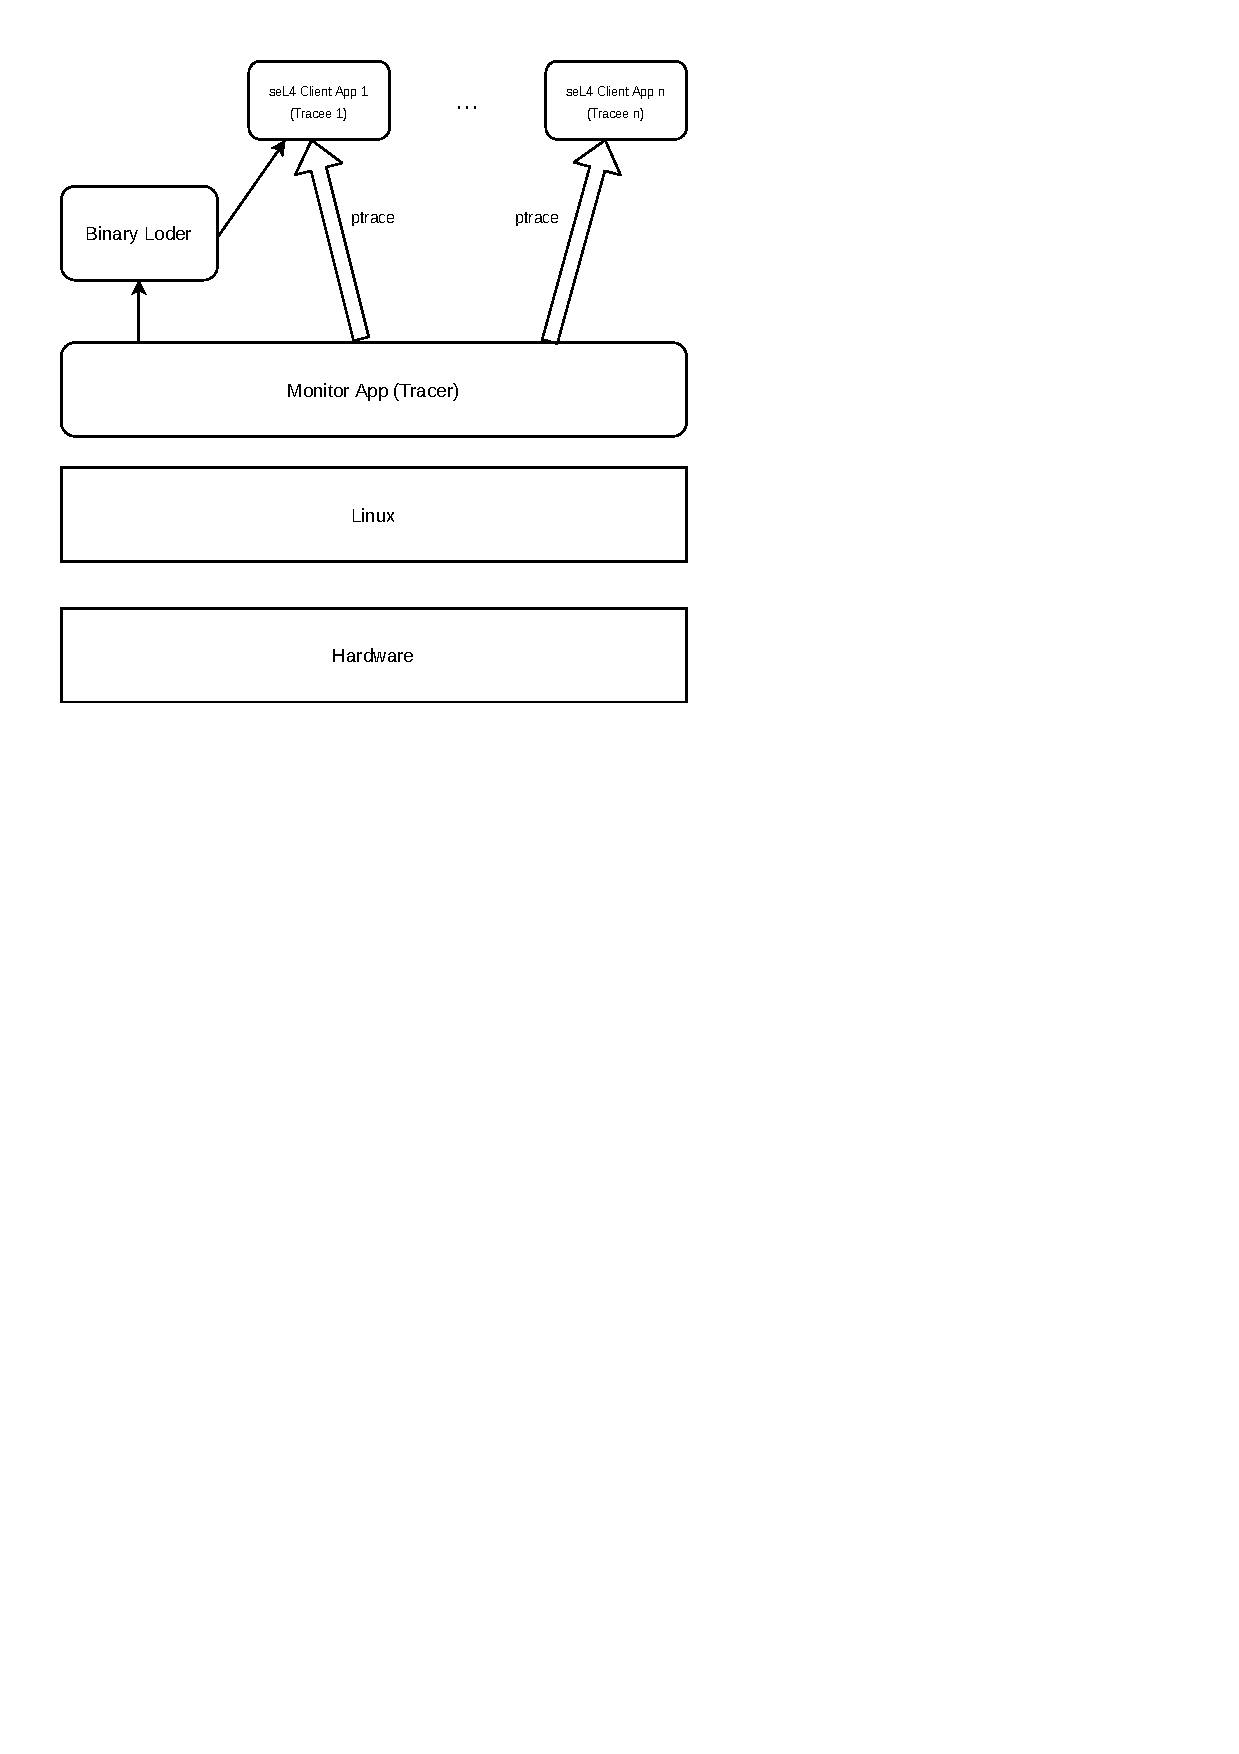
\includegraphics[clip, trim=0.5cm 16cm 8cm 0.5cm, width=0.8\textwidth, height=0.8\textwidth]{ch3/model2-v2.pdf}
    \caption{The model of ABI layer emulation approach}
    \label{fig:mabi}
\end{figure}

Figure \ref{fig:mabi} shows the model of the ABI layer emulation approach.

In the figure, mainly we have two components:

\begin{enumerate}
    \item An seL4 application monitor
    \item An seL4 application binary loader 
\end{enumerate}

In the rest of the article, we will call the seL4 application monitor the \emph{monitor}, and the seL4 application binary loader the \emph{binary loader} for simplicity. The main challenge in this approach is that since the seL4 application is an unmodified binary code, it will invoke the real seL4 system calls. In that case, we have to intercept the system calls and observe what is the seL4 application requesting then serve the system call by ourselves according to the real seL4 semantics. To achieve this goal, we are going to use the $ptrace()$ system call in Linux.

$ptrace()$ allows a tracer process to observe and control the execution of the other process. The "tracee" process can be attached to the "tracer" process, so that the "tracer" can modify the "tracee" process's memory, registers, etc. Also, the $ptrace()$ semantics allow us to establish a one-to-many relationship, which means we can have several "tracees", but can only have one "tracer". In this approach, we can leverage such a feature to intercept the system call invocation from the seL4 applications.

(TODO: Why the loader is requireed and what does the loader do?)

In the model described above, the monitor acts as our "tracer", and the seL4 applications are our "tracees". The monitor is also a seL4 kernel simulator providing the same seL4 semantics and kernel mechanisms as the real seL4 kernel does. The emulation starts from the monitor forks a binary loader process that can load the seL4 application's ELF file into the memory and set up the appropriate memory regions for it. Next, the binary loader will block and notify the monitor that the initialization has finished. The monitor can use $ptrace()$ to control the seL4 application. Finally, the seL4 application can continue executing after the $ptrace()$ process finishes. Now, every time the seL4 application invokes a seL4 system call, the monitor will be notified and suspend the execution of the seL4 application, then the monitor will inspect the system calls requests and do appropriate actions to serve them.

\subsection{Advantages and Disadvantages}
The main advantage of this approach is that the kernel ABI approach is binary compatible. We can directly run an unmodified binary code of seL4 applications without recompilation. However, using the ABI layer emulation will introduce overhead. This is because every time the seL4 application invokes a seL4 system call. The monitor will use $ptrace()$ to intercept it and modify the arguments, return value if necessary, and the $ptrace()$ itself is a system call, which requires trapping into the kernel. The trade-off here is leading to a penalty of the performance. Besides, $ptrace()$ is usually used to implement the Linux debuggers, and it only allows on "tracer" to exist at any time. Therefore, we have to provide our own debugging interfaces in some way, which can introduce implementation complexity.  

\section{Comparison Between API and ABI Layer Emulation}

Table \ref{tb:cmp} listed the trade-offs of implementing the API and the ABI layer emulation approaches. The API layer approach is relatively easier to implement as we don't need to develop the binary loader and the debugging interfaces. The API layer emulation can fully leverage the native Linux debugging tools such as GDB and LLDB. In terms of portability, the API layer approach is ISA compatible as all the implementation is at the seL4 system call library level and doesn't involve the ISA dependent code. However, the API layer approach doesn't achieve binary compatibility as it requires recompiling the source code to work, while the ABI layer emulation approach is fully binary as we intercept the system calls using $ptrace()$.

Last but not least, in terms of the performance, the API layer approach should be better than the ABI layer approach due to the internal implementation. As mentioned before, intercepting system calls and modifying the system calls' arguments or return values require extra context switches to the Linux kernel, which introduces overhead.

\begin{table}[htb]
\centering
\caption{Comparison between API and ABI layer emulation}
\label{tb:cmp}
\resizebox{\textwidth}{!}{\begin{tabular}{llllll}
\hline
Approach &
  \begin{tabular}[c]{@{}l@{}}Implementation\\ Complexity\end{tabular} &
  Portability &
  \begin{tabular}[c]{@{}l@{}}Binary\\ Compatibility\end{tabular} &
  \begin{tabular}[c]{@{}l@{}}Debugging\\ Support\end{tabular} &
  \begin{tabular}[c]{@{}l@{}}Kernel IPC\\ Performance\end{tabular} \\ \hline
\begin{tabular}[c]{@{}l@{}}Syscall Library\\ API emulation\end{tabular} &
  Intermediate &
  \begin{tabular}[c]{@{}l@{}}Good, as the \\ solution is ISA \\ portable\end{tabular} &
  No &
  \begin{tabular}[c]{@{}l@{}}Can use native \\ Linux debugging \\ tools\end{tabular} &
  First \\
\begin{tabular}[c]{@{}l@{}}Kernel ABI \\ emulation\end{tabular} &
  Difficult &
  \begin{tabular}[c]{@{}l@{}}No, if the ABI of \\ the application is different \\ from the host's,\\ it won't work\end{tabular} &
  Yes &
  \begin{tabular}[c]{@{}l@{}}Extra debugging\\ interface required\end{tabular} &
  Second \\ \hline
\end{tabular}}
\end{table}

% (Fixed: why ABI emulation approach is ISA independent, It is not as the ELF file will be different, in this project targeting to x86)